% Name: Möbius strip
% Description: A Möbius strip drawn as a surface: a band with a half twist, so it has only one side and one edge.
% Tags: Möbius strip, non-orientable surface, topology, pgfplots

\usepackage{pgfplots}
\pgfplotsset{compat=1.18}

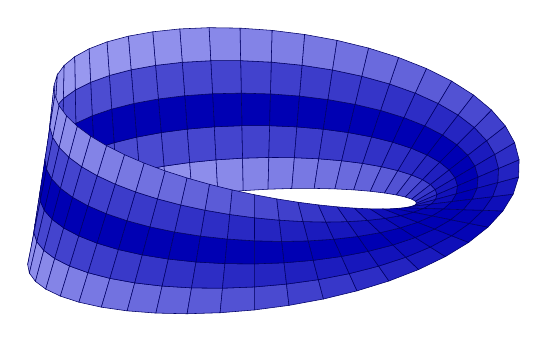
\begin{tikzpicture}
  \begin{axis}[hide axis, view={30}{40}, width=10cm, height=7cm, colormap={band}{color=(blue!25) color=(blue!70!black) color=(blue!25)}, z buffer=sort]
    % (1 + (v/2) cos(u/2)) (cos u, sin u) and height (v/2) sin(u/2): the cross-section turns half a turn as u goes once round
    \addplot3[surf, faceted color=blue!40!black, line width=0.2pt, domain=0:360, y domain=-0.5:0.5, samples=48, samples y=6]
      ({(1 + y/2*cos(x/2))*cos(x)}, {(1 + y/2*cos(x/2))*sin(x)}, {y/2*sin(x/2)});
  \end{axis}
\end{tikzpicture}
